\documentclass[11pt, letterpaper]{article}
\usepackage[utf8]{inputenc}
\usepackage{geometry}
\usepackage{fancyhdr}
\usepackage{amsmath, amssymb}
\usepackage{xcolor}
\usepackage{listings}
\usepackage{enumitem}
\usepackage{hyperref}
\usepackage{booktabs}
\usepackage{graphicx}

% Make parindent 0
\setlength{\parindent}{0pt}
\setlist{itemsep=0.5em}
\setlength{\parskip}{0.5em}

\geometry{margin=1in}
\setlength{\headheight}{14pt}
\pagestyle{fancy}
\fancyhf{}
\lhead{\textbf{Solutions}}
\rhead{\textbf{Data Analysis and Regression, Homework 1}}
\cfoot{\thepage}

\definecolor{codegreen}{rgb}{0,0.6,0}
\definecolor{codegray}{rgb}{0.5,0.5,0.5}
\definecolor{codepurple}{rgb}{0.58,0,0.82}
\definecolor{backcolour}{rgb}{0.95,0.95,0.92}

\lstdefinestyle{mystyle}{
    backgroundcolor=\color{backcolour},   
    commentstyle=\color{codegreen},
    keywordstyle=\color{magenta},
    numberstyle=\tiny\color{codegray},
    stringstyle=\color{codepurple},
    basicstyle=\ttfamily\footnotesize,
    breakatwhitespace=false,         
    breaklines=true,                 
    captionpos=b,                    
    keepspaces=true,                 
    numbers=left,                    
    numbersep=5pt,                  
    showspaces=false,                
    showstringspaces=false,
    showtabs=false,                  
    tabsize=2
}
\lstset{style=mystyle}

\newcommand{\problem}[1]{\section*{Problem #1}}
\newcommand{\subproblem}[1]{\subsection*{Problem #1}}
\newcommand{\answer}{\textbf{\textit{\textcolor{red}{Answer:}}}\\}

\begin{document}

\section*{Instructions}
\begin{itemize}
    \item Homework 1 was due Monday, July 27th at 18:00 Chicago Time.
    \item All numbers and figures come from \texttt{homework\_1\_solution.ipynb}, run from top to bottom.
\end{itemize}
\hrule
\vspace{0.5cm}

\pagebreak

\problem{1: One-Dimensional Data}

Load in the data from the GitHub repository for this class.
\begin{lstlisting}[language=python]
import pandas as pd

df = pd.read_csv(
    "https://raw.githubusercontent.com/tobiasdelpozo/data-analysis-2026/refs/heads/master/homework/homework_1/questions/homework_1_data.csv"
)
\end{lstlisting}

\subproblem{1.1}

For the feature labeled \texttt{X1}, compute the mean, median, variance, and standard deviation. 
Report your numbers below (rounded to at least 4 decimal places).

\answer
\begin{center}
\begin{tabular}{lr}
\toprule
 & Value \\
\midrule
mean & 12.3435 \\
median & 11.9216 \\
variance & 38.8894 \\
std & 6.2361 \\
\bottomrule
\end{tabular}
\end{center}


\subproblem{1.2}

Display a histogram of the feature \texttt{X1} using 50 bins. Do you think that 
the statistics you computed in 1.1 are good descriptors of the data? Include the graph below,
and explain your reasoning in 1-2 sentences. \footnote{Hint: you can use \texttt{\textbackslash includegraphics\{\}} to include images in \LaTeX.}

\answer
No. The data has three peaks, at roughly $5$, $12$ and $20$, each holding about a third of the
points. The mean and the median land on the middle peak and say nothing about the other two, and
the standard deviation of $6.2361$ measures the gaps between the peaks rather than the spread
within any one of them.

\begin{center}
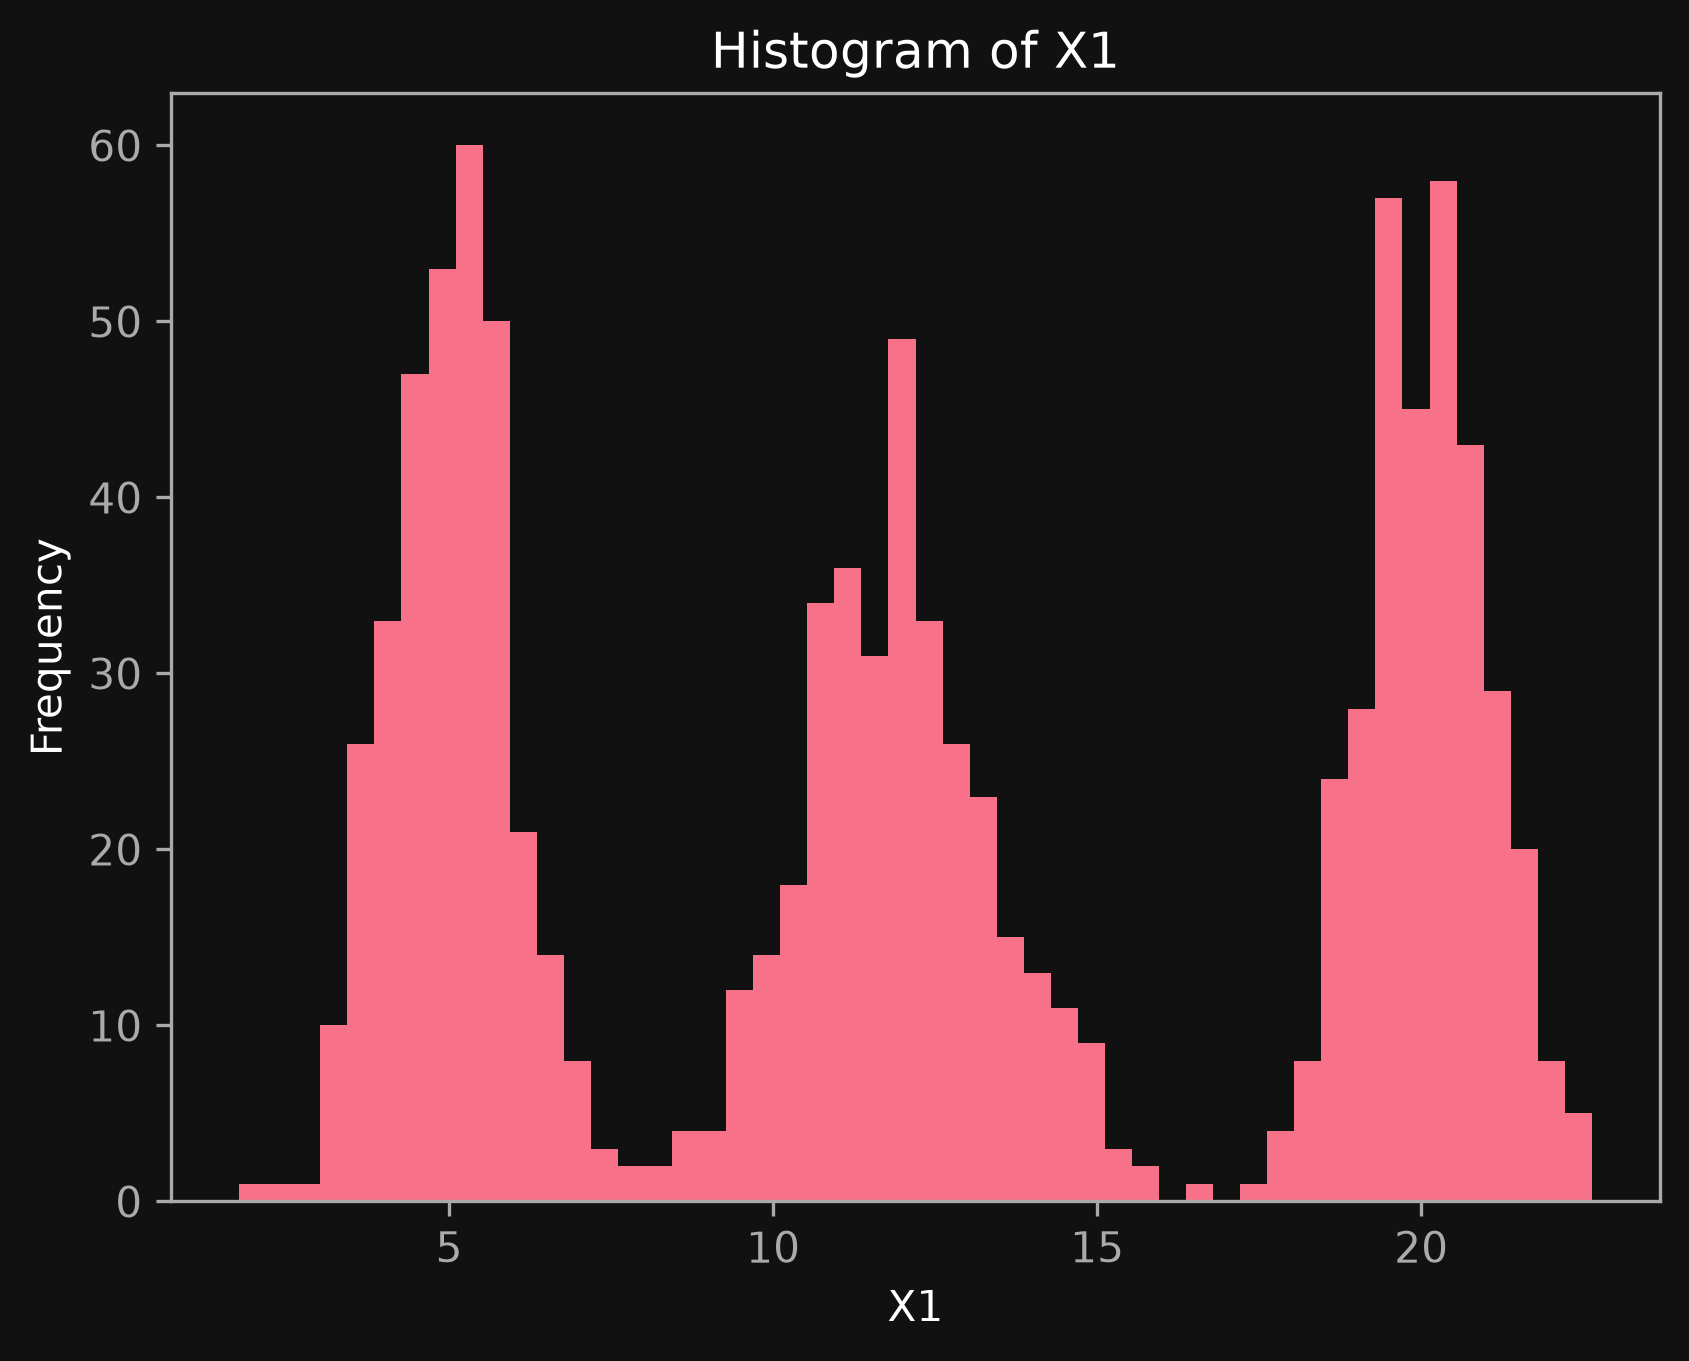
\includegraphics[width=0.58\textwidth]{./figures/problem1_histogram.png}
\end{center}


\subproblem{1.3}

Using the same feature \texttt{X1}, come up with some metrics that 
are descriptive of the distribution of the data. Note, this is open-ended,
so think about what the data looks like, and how a human would describe it.

\answer
Take the local maxima of a kernel density estimate as the modes, then assign each point to its
nearest mode and describe the three groups separately.

\begin{center}
\begin{tabular}{lrrrr}
\toprule
cluster & mode & mean & std & share \\
\midrule
0 & 5.0392 & 5.0368 & 0.9878 & 0.3320 \\
1 & 11.8508 & 11.9600 & 1.4572 & 0.3370 \\
2 & 20.0624 & 20.0628 & 0.9787 & 0.3310 \\
\bottomrule
\end{tabular}
\end{center}

Within a cluster the standard deviation is about $1$, against the $6.2361$ of 1.1. Four numbers per
mode, plus the three shares, describe the data; one mean does not.



\pagebreak

\problem{2: kNN Regression}

This problem uses the same dataset as Problem 1.

We're going to implement a k-Nearest Neighbors regression model. Unless otherwise specified, use an 80/20 train/test split for all parts of this problem.

\subproblem{2.1}

Display a plot of \texttt{X2} versus the \texttt{target} variable. What 
do you notice about the relationship between these two variables?

\answer
The relationship is not linear. The target rises and falls three times across the range of
\texttt{X2}, peaking near $X2 = 3$, $7.5$ and $12$, and the noise around that shape is small.

\begin{center}
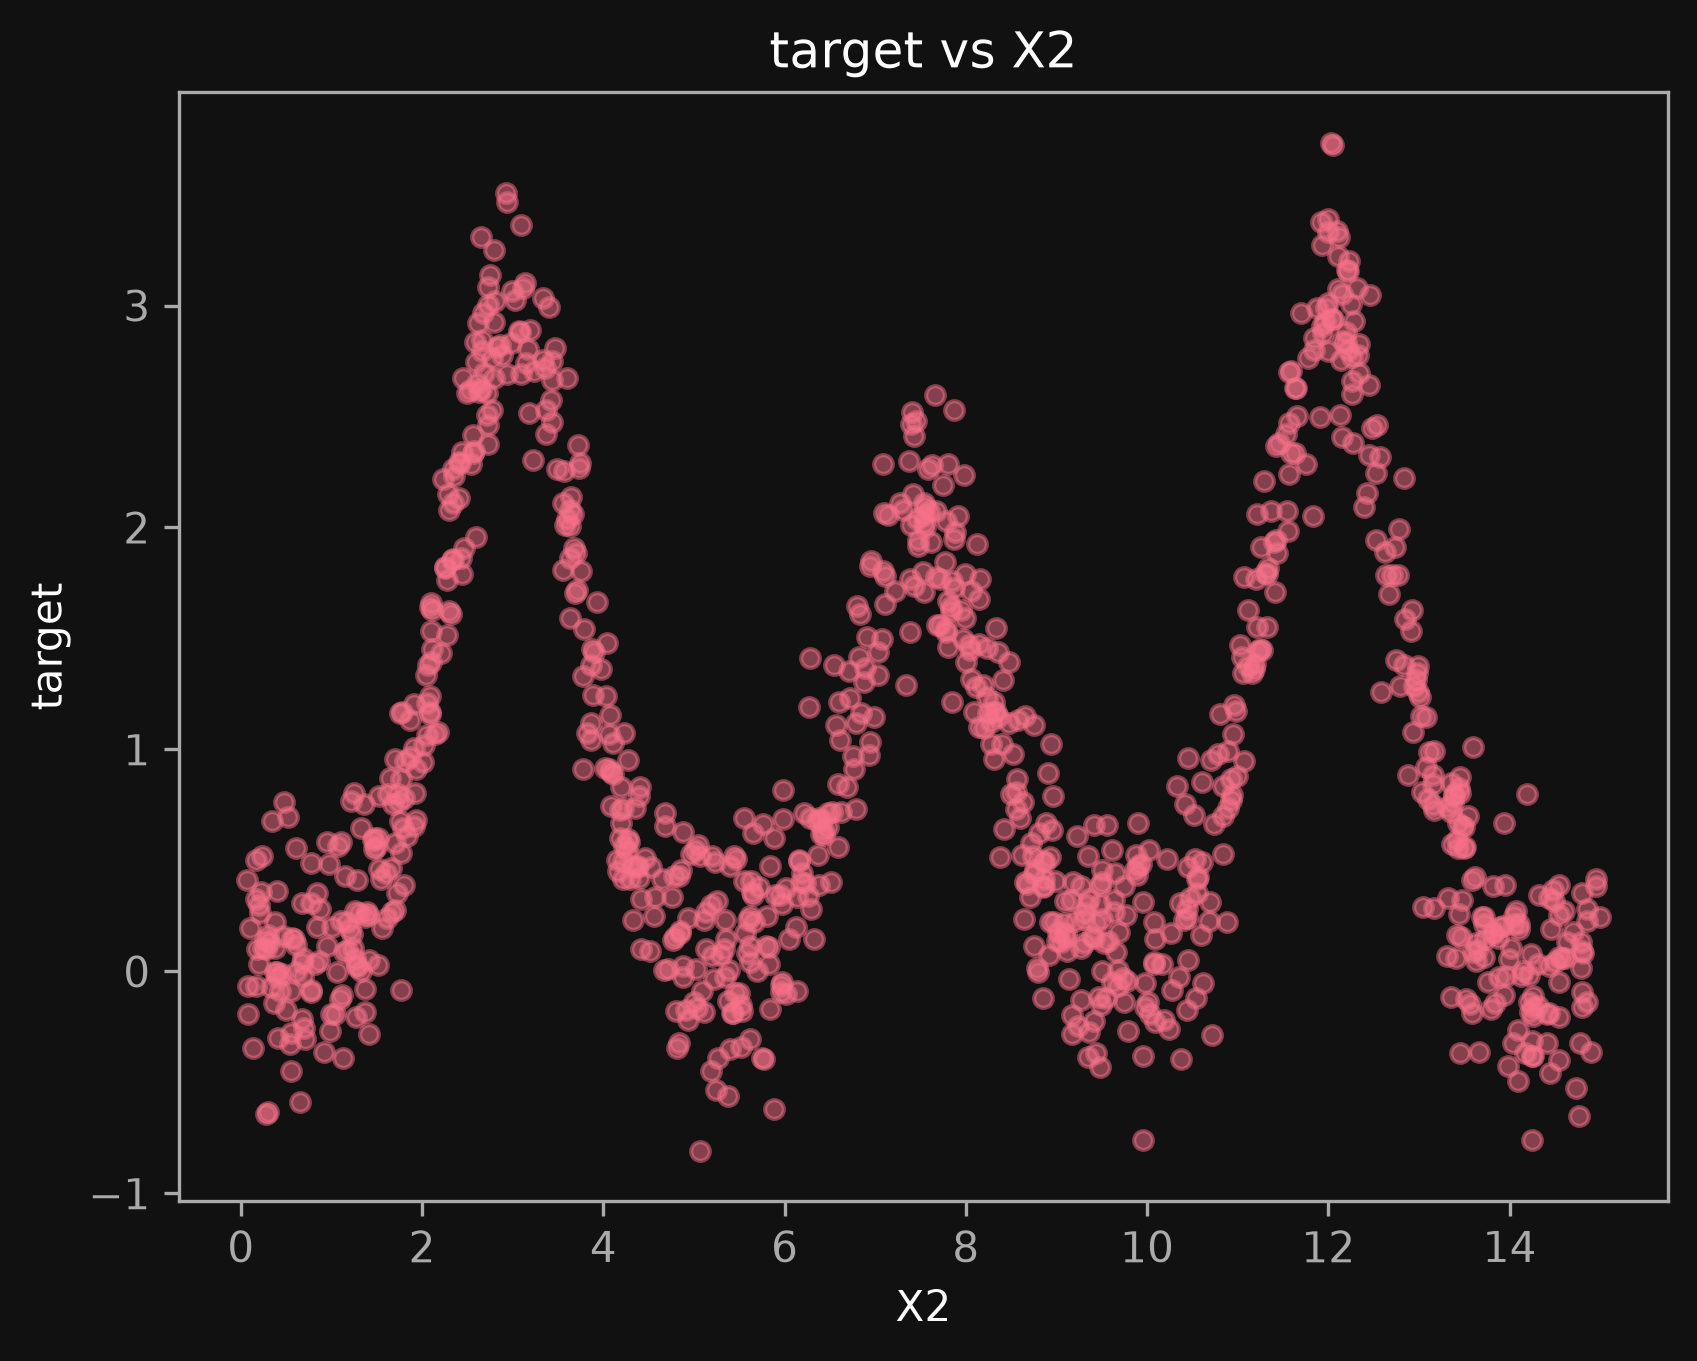
\includegraphics[width=0.58\textwidth]{./figures/problem2_scatter.png}
\end{center}


\subproblem{2.2}

Implement a kNN regression model from scratch. You may use \texttt{numpy} and \texttt{pandas}, but you may not use any machine learning libraries (e.g. \texttt{scikit-learn}).

Your model should take in 4 parameters:
\begin{itemize}
    \item \texttt{X\_train}: training features
    \item \texttt{y\_train}: training target variable
    \item \texttt{X\_test}: testing features
    \item \texttt{k}: number of neighbors to use
\end{itemize}
And it should output the predicted values for \texttt{X\_test}.

The algorithm you should use is as follows:
\begin{enumerate}
    \item For each test point, compute the Euclidean distance to all training points.
    \item Identify the k-nearest neighbors based on these distances.
    \item Compute the predicted value as the mean of the target variable of these k-nearest neighbors.
\end{enumerate}
Note that we are only considering a single feature for this problem, so the Euclidean distance is
simply $\sqrt{(x_{\text{test}} - x_{\text{train}})^2}$.

Include your code implementation below.\footnote{
    Hint: you can use \texttt{\textbackslash lstlisting[language=python]} to include Python code snippets.
}

\answer
Two implementations. The first loops over test points; the second does the whole distance matrix at
once, which is faster but costs $n_{\text{train}} \times n_{\text{test}}$ memory.

\begin{lstlisting}[language=Python]
def knn_regressor(X_train, y_train, X_test, k):
    y_pred = []
    for x_test in X_test:
        distances = np.linalg.norm(X_train - x_test, axis=1)
        knn_indices = np.argsort(distances)[:k]
        y_pred.append(np.mean(y_train[knn_indices]))
    return np.array(y_pred)


def knn_regressor_matrix(X_train, y_train, X_test, k):
    distances = np.linalg.norm(X_train[:, np.newaxis] - X_test[np.newaxis, :], axis=2)
    knn_indices = np.argsort(distances, axis=0)[:k, :]
    return np.mean(y_train[knn_indices], axis=0)
\end{lstlisting}

The two agree to floating point on this data.


\subproblem{2.3}

Randomly split the data into training and testing sets (80/20 split), and
report the Mean Squared Error (MSE) of your kNN regression model on the test set for $k=5$.

\answer
$\text{MSE} = 0.0996$ at $k = 5$.

\begin{lstlisting}[language=Python]
np.random.seed(42)

ind = df.index.to_numpy().copy()
np.random.shuffle(ind)
n = len(ind)
train_ind, test_ind = ind[: int(n * 0.8)], ind[int(n * 0.8) :]

X_train = df.loc[train_ind, ["X2"]].to_numpy()
X_test = df.loc[test_ind, ["X2"]].to_numpy()
y_train = df.loc[train_ind, "target"].to_numpy()
y_test = df.loc[test_ind, "target"].to_numpy()

y_pred = knn_regressor(X_train, y_train, X_test, k=5)
mse = ((y_test - y_pred) ** 2).mean()
\end{lstlisting}


\subproblem{2.4}

For $k \in \{1, 5, 10, 20, 50, 100 \}$, compute the MSE on the test set and plot the results (k values on the x-axis, MSE on the y-axis).
What value of $k$ gives the best performance on the test set?

\answer
$k = 20$, at $\text{MSE} = 0.0926$.

\begin{center}
\begin{tabular}{rr}
\toprule
$k$ & test MSE \\
\midrule
1 & 0.1838 \\
5 & 0.0996 \\
10 & 0.0939 \\
20 & \textbf{0.0926} \\
50 & 0.0995 \\
100 & 0.1740 \\
\bottomrule
\end{tabular}
\end{center}

\begin{center}
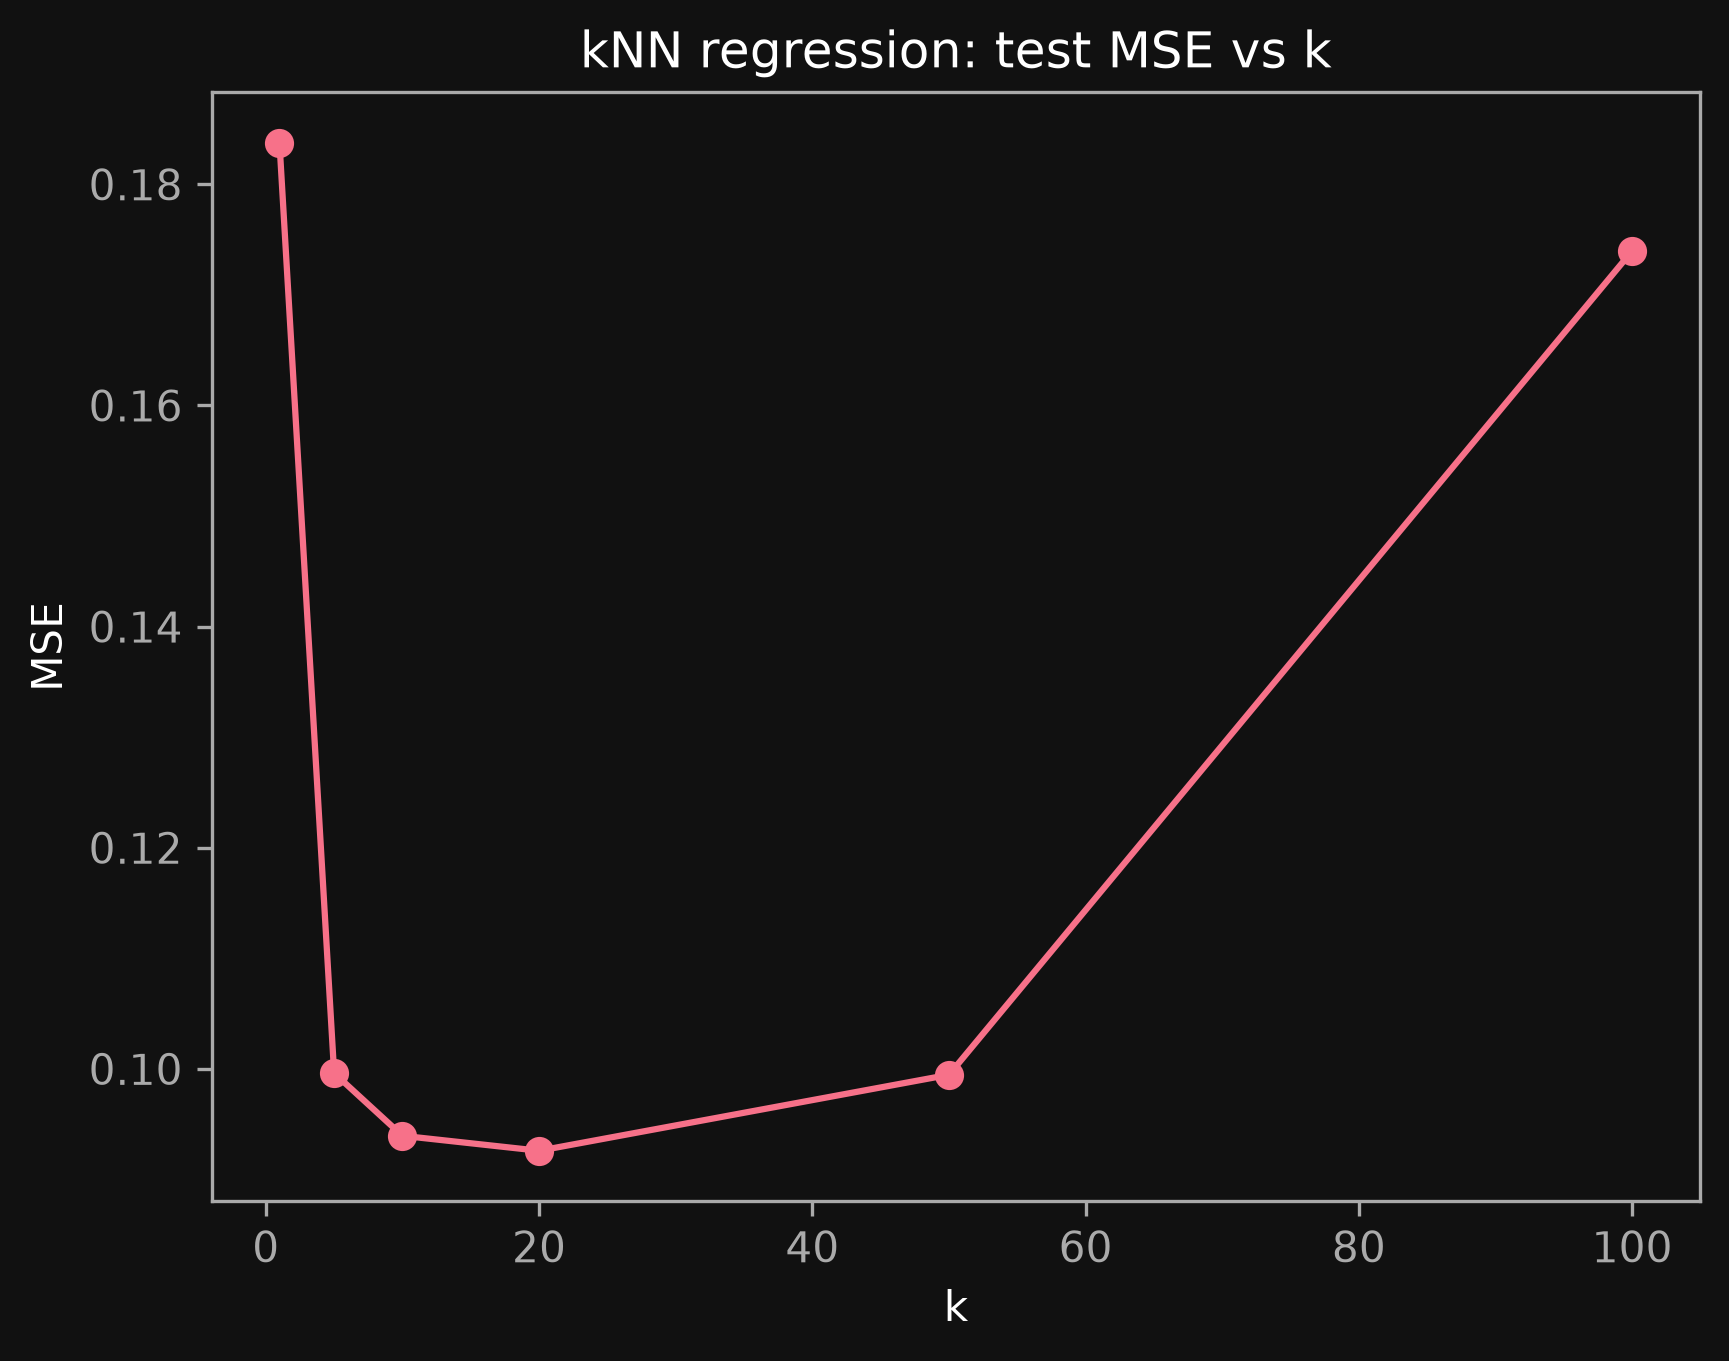
\includegraphics[width=0.58\textwidth]{./figures/problem2_mse_vs_k.png}
\end{center}



\subproblem{2.5}

Which value of $k$ do you think has the highest bias? And which has the highest variance? Explain your reasoning in 1-2 sentences.

\answer
$k = 100$ has the highest bias. It averages an eighth of the 800 training points for every
prediction, which flattens the three peaks of 2.1 into something close to the overall mean.

$k = 1$ has the highest variance. Each prediction is a single training point, so it carries that
point's noise in full.

Both sit at the ends of the table above, and both are worse than $k = 20$.


\problem{3: Linear Regression}

Using the same dataset as Problems 1 and 2, we are going to explore linear regression.

\subproblem{3.1}

Using \texttt{statsmodels}, fit a linear regression model to predict \texttt{y} using \texttt{X3}.
You should \textbf{not} use an intercept term in your model. Report your
$\beta$ coefficient below:

\answer
$\hat{\beta} = 0.5642$.


\subproblem{3.2}

Re-run the linear regression model from 3.1, but this time include an intercept term.
What are your new $\beta$ coefficients (intercept and slope)?

\answer
$\hat{\beta}_0 = 7.1515$ and $\hat{\beta}_1 = -0.2926$, with $R^2 = 0.1707$.

The slope changes sign once the intercept is free. Without an intercept the line is forced through
the origin, and since $y$ is around $5$ everywhere, the only way to fit it is with a positive slope.


\subproblem{3.3}

Do the following data transformations:
$$\tilde{y} = y - \bar{y} \quad \quad \tilde{X}_3 = X_3 - \bar{X}_3$$

Re-run the linear regression model using $\tilde{y}$ and $\tilde{X}_3$, without an intercept term.
What is your $\beta$ coefficient? How does it compare to your answer in 3.1?

\answer
$\hat{\beta} = -0.2926$. This does not match 3.1, but it matches the slope in 3.2 exactly.

Centering is the same thing as fitting an intercept. The OLS intercept is
$$
\hat{\beta}_0 = \bar{y} - \hat{\beta}_1 \bar{X}_3,
$$
so subtracting the means from both sides leaves a model whose intercept is zero by construction.


\subproblem{3.4}

Inspect your data. Display a scatter plot of \texttt{X3} versus \texttt{y}. What do you notice about the relationship between these two variables?
Is a linear model appropriate for this data? Explain your reasoning in 1-2 sentences.

\answer
The relationship is periodic: $y$ runs through two full cycles between $5$ and $9$ as $X_3$ goes
from $0$ to about $4\pi$. A straight line cannot follow that, which is why 3.2 explains only
$17\%$ of the variance.

\begin{center}
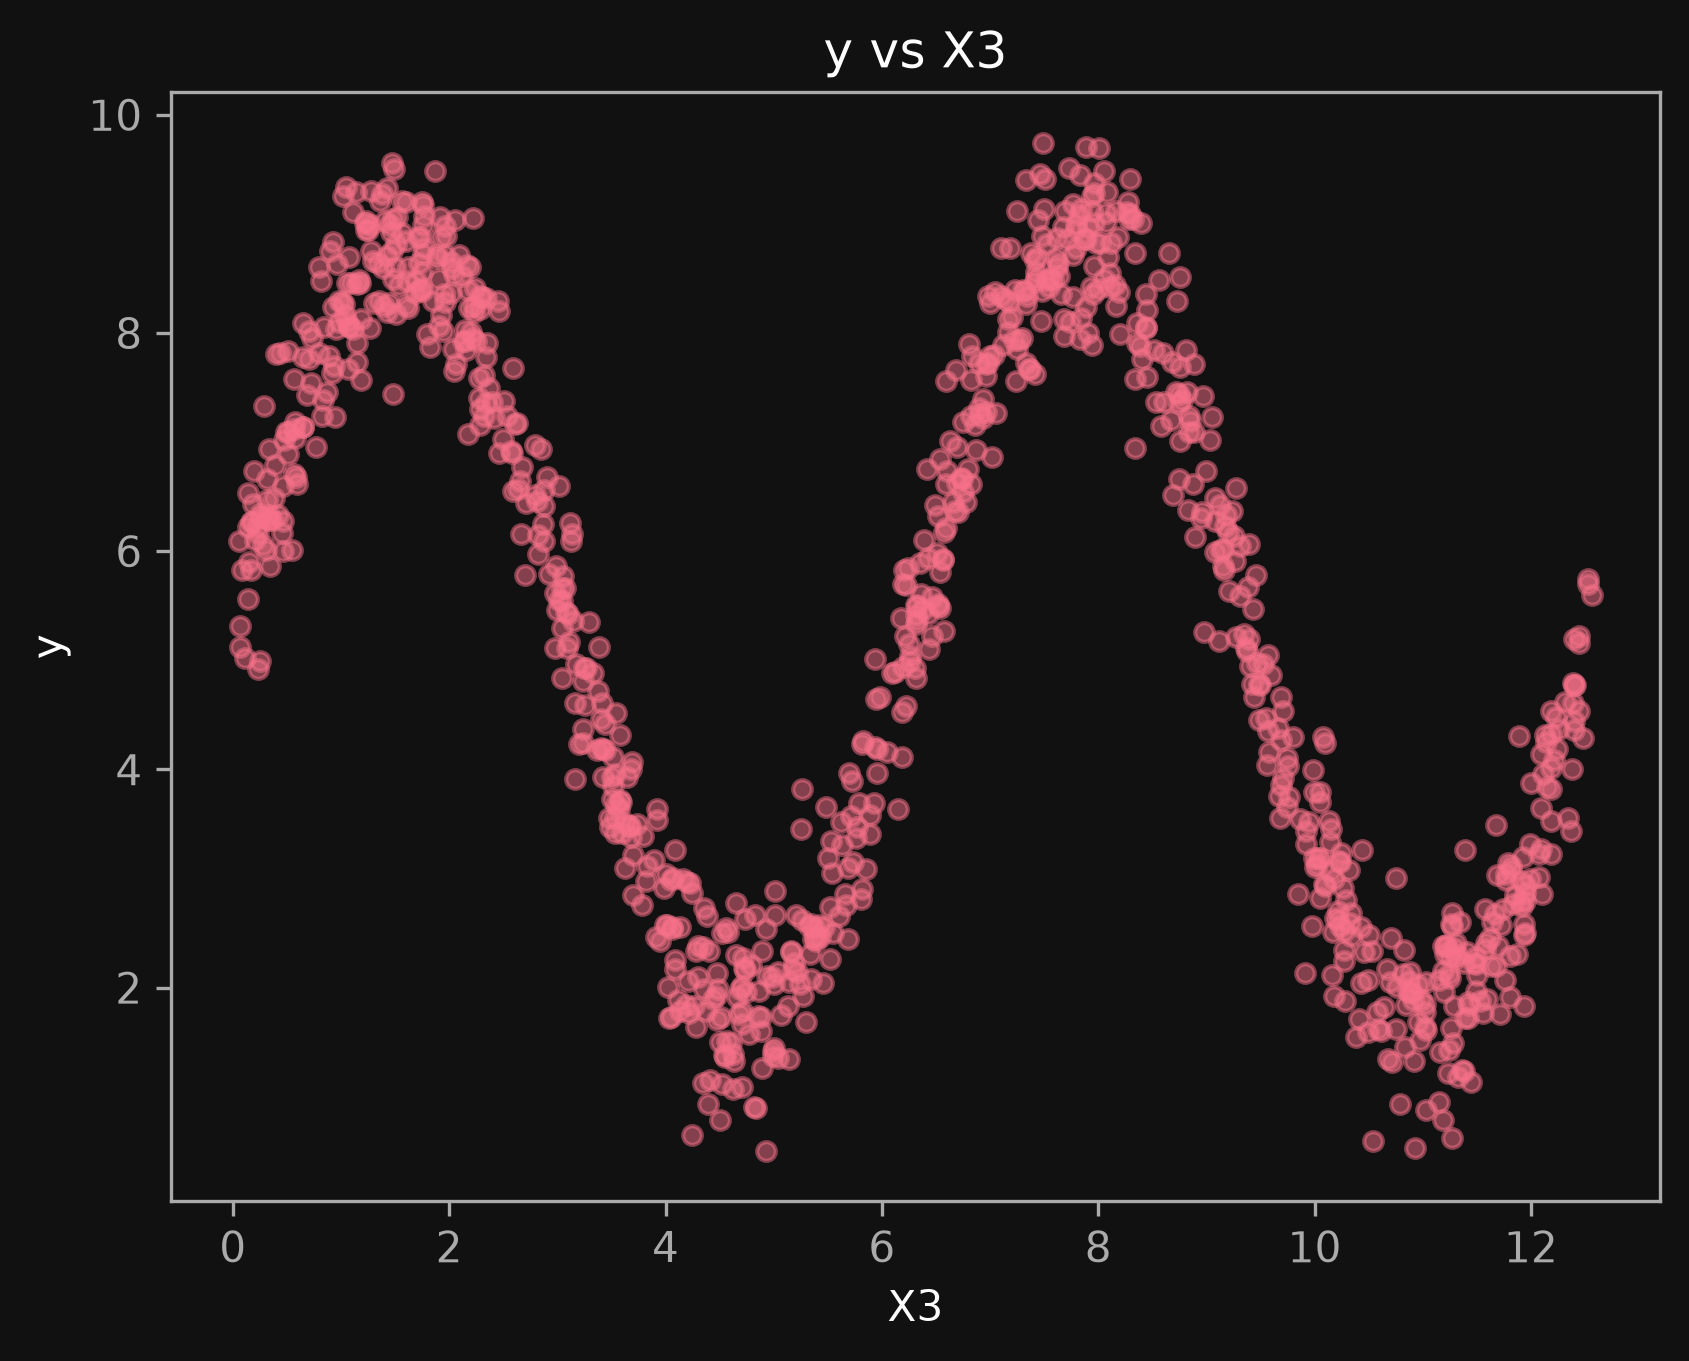
\includegraphics[width=0.58\textwidth]{./figures/problem3_scatter.png}
\end{center}


\subproblem{3.5}

Define a new feature $\texttt{X3\_sin}$ as follows: 
$$\texttt{X3\_sin} = \sin(\texttt{X3})$$

Fit a linear regression model to predict \texttt{y} using \texttt{X3\_sin}, including an intercept term.
Report your $\beta$ coefficients (intercept and slope) below:

\answer
$\hat{\beta}_0 = 5.2484$ and $\hat{\beta}_1 = 3.5362$, with $R^2 = 0.9639$ against the $0.1707$ of
3.2.


\subproblem{3.6}

Display a plot of \texttt{X3\_sin} versus \texttt{y}. Do you think a linear model is appropriate for this data? Explain your reasoning in 1-2 sentences.

\answer
Yes. The transformation makes the relationship linear, which is the point: the model is still
linear in its coefficients, and all we changed was the feature.

\begin{center}
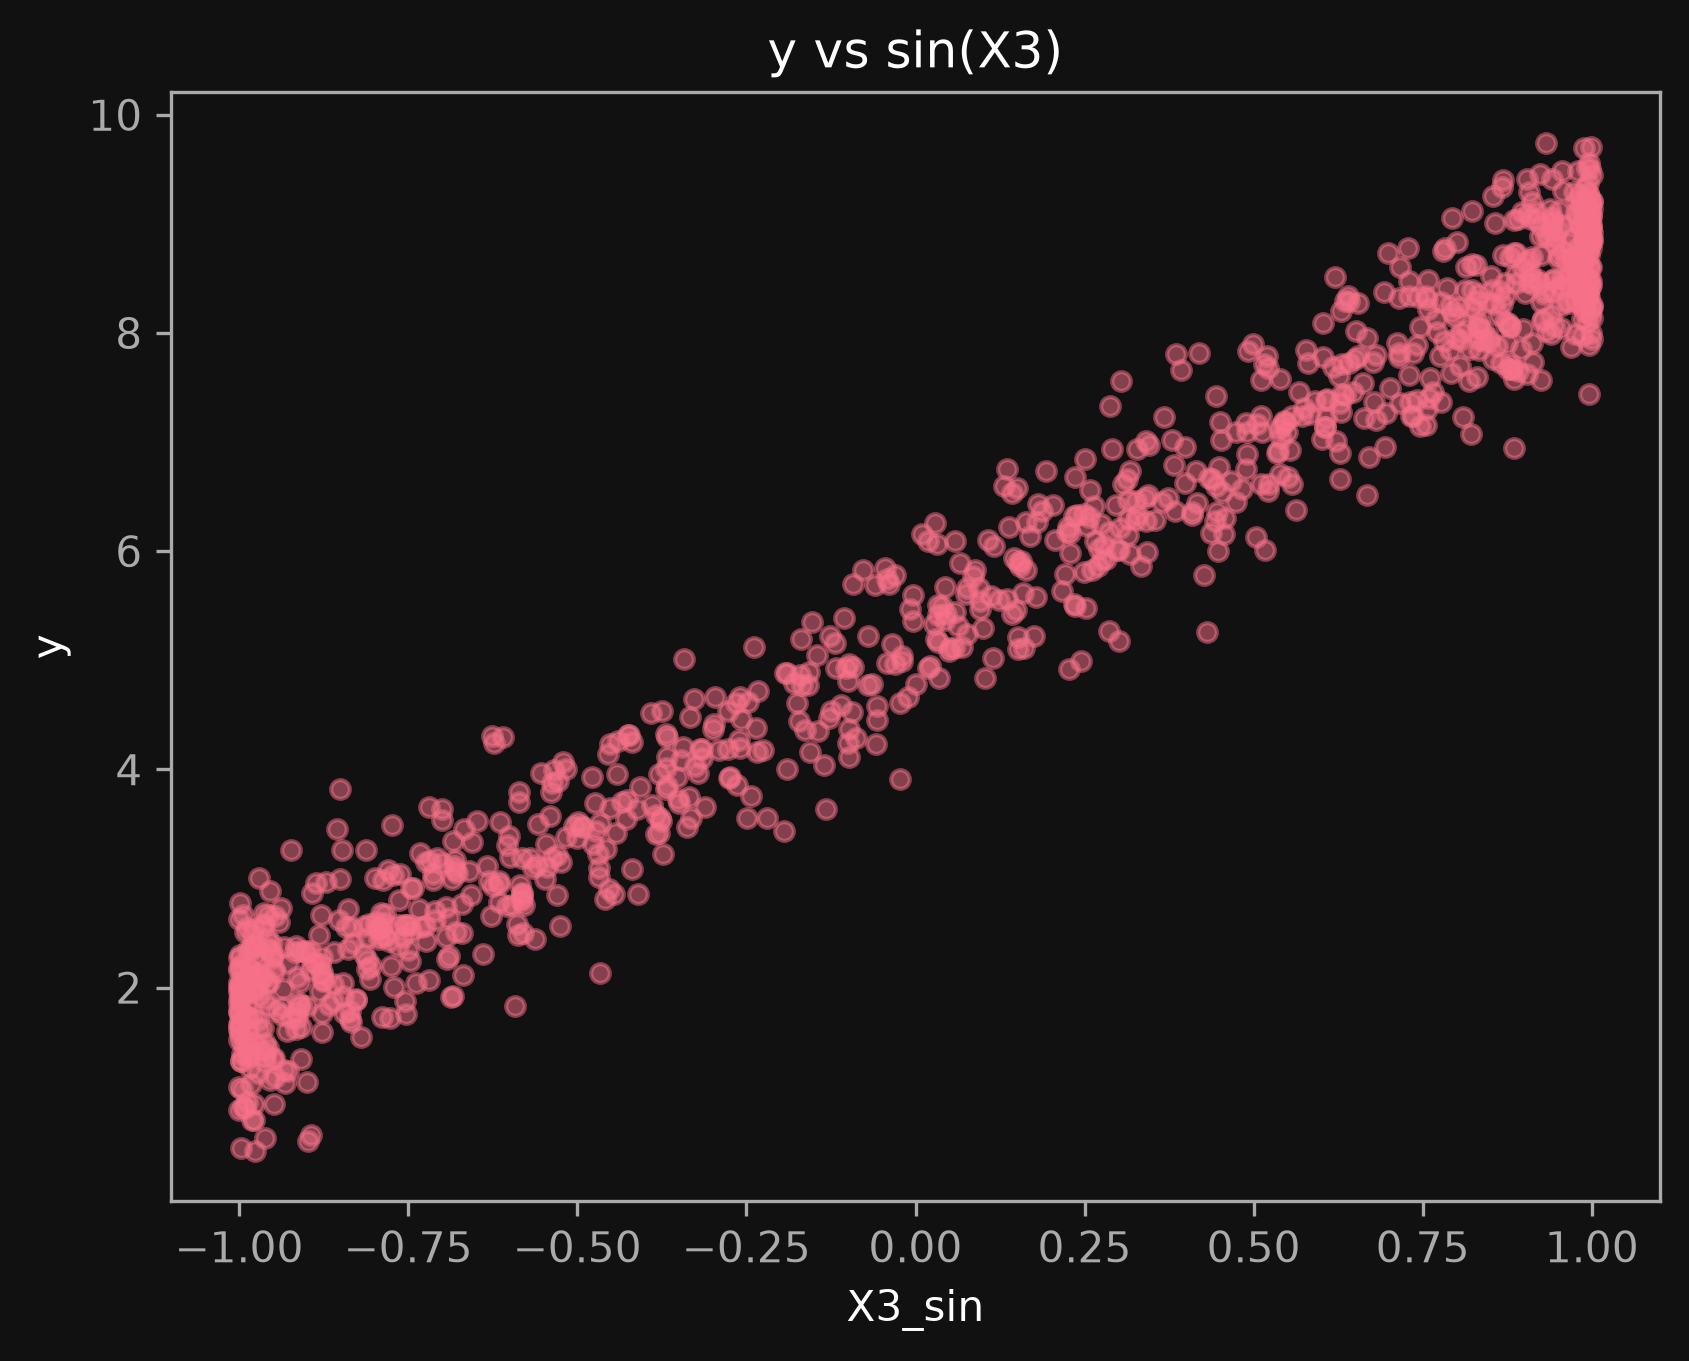
\includegraphics[width=0.58\textwidth]{./figures/problem3_scatter_sin.png}
\end{center}


\end{document}